\documentclass[brudnopis]{xmgr}

%\defaultfontfeatures{Scale=MatchLowercase}
%\setmainfont[Numbers=OldStyle,Ligatures=TeX]{Minion Pro}
%\setsansfont[Numbers=OldStyle,Ligatures=TeX]{Myriad Pro}
% for fontspec version < 2.0
\setmainfont[Numbers=OldStyle,Mapping=tex-text]{Minion Pro}
\setsansfont[Numbers=OldStyle,Mapping=tex-text]{Myriad Pro}
%\setmonofont[Scale=0.75]{Monaco}

% Opcjonalnie identyfikator dokumentu
% drukowany tylko z włączoną opcją 'brudnopis':
\wersja   {wersja wstępna [\ymdtoday]}

\author   {Michał Dettlaff}
\nralbumu {164\,622}
\email    {walenty@szczesny.com.pl}

\title    {Zastosowanie algorytmów genetycznych w projektowaniu optymalnego układu klawiatury}
\date     {2011}
\miejsce  {Gdańsk}

\opiekun  {prof. zw. dr hab. inż. Sławomir Wierzchoń}

% dodatkowe polecenia
%\renewcommand{\filename}[1]{\texttt{#1}}

\begin{document}

\begin{abstract}
  Projektowanie optymalnego, ergonomicznego układu klawiatury można potraktować jako problem optymalizacyjny, do rozwiązania którego można zastosować znane metaheurystyki. W poniższej pracy wykorzystany jest do tego celu algorytm genetyczny, w którym genotyp stanowi układ klawiszy zakodowany jako permutacja, a funkcja przystosowania odzwierciedla ilość pracy potrzebną do przepisania tekstu za pomocą danego układu. W wyniku zostają utworzone układy klawiatury przystosowane do pisania w języku polskim oraz angielskim, które następnie są porównane ze standardowymi układami klawiatury (QWERTY, Dvorak), zaprojektowanymi bez udziału komputera.
\end{abstract}
\keywords{
  algorytmy, genetyczne, Dvorak, QWERTY, optymalizacja
}

% tytuł i spis treści
\maketitle
%
% wstęp
\introduction

Standardowy układ klawiatury (rys. 1), mimo swojej wszechobecności oraz pozostawania w użyciu od ponad 100 lat, jest pod wieloma względami nieoptymalny. Układ ten nazywany jest układem QWERTY (od pierwszych liter w górnym rzędzie w jego amerykańskiej wersji) lub układem Scholesa i został zaprojektowany w latach 70 XIX wieku przez Charles'a Lethama Sholesa. QWERTY zastąpił używany wcześniej układ alfabetyczny i miał na celu zapobieganie zacinaniu się mechanizmu maszyny do pisania, jeżeli użytkownik pisał zbyt szybko~\cite{Norman:1988:DOET}. Z tego względu, litery które często występowały obok siebie w języku angielskim, takie jak \emph{i} oraz \emph{e}, zostały umieszczone po przeciwnych stronach klawiatury. Dzięki temu, belki na których znajdowały się klawisze nie zderzały się ze sobą, co zmniejszało prawdopodobieństwo zacięcia się. Mimo że problem zacinania się maszyny został szybko wyeliminowany i to jeszcze na długo przed nadejściem klawiatury komputerowej, układ klawiatury QWERTY pozostaje w użyciu aż do dzisiaj.

\begin{figure}[!tbh]
\centering
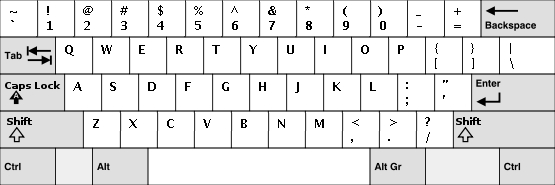
\includegraphics[width=.8\hsize]{fig/qwerty}
\caption{Standardowy układ klawiatury QWERTY}
\source{Opracowanie własne}
\end{figure}

Spośród układów alternatywnych wobec QWERTY największą popularnością cieszy się klawiatura Dvoraka (Dvorak Simplified Keyboard). Została ona zaprojektowana w 1936 r. przez dr Augusta Dvoraka. W przeciwieństwie do QWERTY, podczas jej projektowania nie były już brane pod uwagę ograniczenia mechaniczne maszyn do pisania, ze względu na postępy w ich produkcji. Głównym celem było natomiast umożliwienie efektywnego pisania oraz łatwość nauki. W tym celu zostały wzięte pod uwagę takie czynniki jak częstotliwości występowania liter oraz poziom wykorzystania najłatwiej dostępnego, środkowego rzędu klawiszy. Dla przykładu, za pomocą samego środkowego rzędu klawiatury Dvoraka można napisać około 400 słów w języku angielskim, natomiast układ QWERTY pozwala w analogiczny sposób napisać tylko około 100 słów~\cite{Call:2005:CME}. Klawiatura Dvoraka jest łatwiejsza w nauce i pozwala na około 10\% szybsze pisanie~\cite{Norman:1988:DOET}.

\begin{figure}[!tbh]
\centering
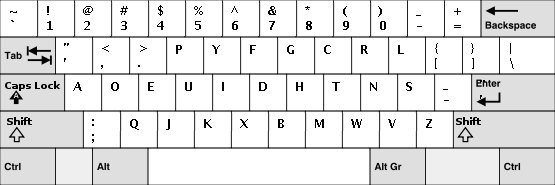
\includegraphics[width=.8\hsize]{fig/dvorak}
\caption{Układ klawiatury Dvorak Simplified Keyboard}
\source{Opracowanie własne}
\end{figure}


\chapter{Metodologia}

Algorytmy genetyczne.

\chapter{Opis algorytmu}


\section{Reprezentacja genotypu}

Stosowana jest permutacyjna reprezentacja genotypu. Układ klawiatury reprezentowany jest przez permutację 30 klawiszy. 26 klawiszy oznaczanych jest literami alfabetu łacińskiego A-Z, a pozostałe odpowiadają znakom {\tt ,}, {\tt .}, {\tt ?} oraz {\tt ;}. Wynika z tego, że liczba wszystkich możliwych układów klawiatury wynosi $$ 30! = 2.7 * 10^{32} $$ co stanowi rozmiar przestrzeni poszukiwań na której będzie działał algorytm genetyczny. Zbiór wszystkich znaków wchodzących w skład permutacji oznaczymy jako $ A $.

Klawisze podzielone są na trzy grupy, gdzie pierwsze 10 oznacza klawisze górnego rzędu klawiatury, następne 10 klawisze rzędu środkowego, a ostatnie 10 - dolnego rzędu.

Dla przykładu, układ klawiatury QWERTY jest reprezentowany przez następującą permutację:
$$ qwertyuiopasdfghjkl;zxcvbnm,.? $$


\section{Funkcja przystosowania}

Naszym celem jest znalezienie układu klawiatury, który przyczyni się do zwiększenia prędkości pisania oraz zminimalizowania zmęczenia palców użytkownika. Inne pożądane cechy to minimalizowanie ilości błędów oraz łatwość nauki danego układu klawiatury. Dlatego też te cele będą brane pod uwagę podczas projektowania funkcji przystosowania algorytmu genetycznego.

W kolejnych podrozdziałach zostaną opisane kryteria, które składają się na funkcję przystosowania. Ostateczna postać funkcji przystosowania jest sumą ważoną wyników z poszczególnych kryteriów.

Do obliczania oceny układu klawiatury wykorzystywane są zbiory tekstów, stanowiących możliwie reprezentatywną próbkę z danego języka. Wynikowy układ powinien być jak najlepiej przystosowany do przepisywania podanego tekstu, dlatego użyte zostaną osobne zbiory tekstów dla języka polskiego oraz angielskiego. Naiwnym sposobem na obliczenie przystosowania byłaby symulacja przepisywania tekstu, wymagająca analizy całości tekstu za każdym razem od nowa podczas obliczania funkcji przystosowania. Takie podejście jest jednak zbyt kosztowne obliczeniowo, ponieważ złożoność funkcji przystosowania wyniosłaby $ O(n) $, gdzie $ n $ stanowiące długość tekstu byłoby wartością rzędu $ 10^5 $ lub $ 10^6 $.

Z tego powodu funkcja przystosowania nie będzie obliczana na podstawie oryginalnego tekstu, ale jego cech statystycznych, które będą obliczane tylko raz przed uruchomieniem algorytmu. W ten sposób czas obliczania funkcji przystosowania nie będzie zależny od długości tekstu (jego złożoność wyniesie $ O(1) $). Cechy statystyczne tekstu zostaną opisane za pomocą dwóch funkcji:
$$ f_m : M \rightarrow \mathrm{R} $$
$$ f_d : D \rightarrow \mathrm{R} $$

Dziedzinę funkcji $ f_m $ będziemy określać jako zbiór monografów $ M $ (pojedynczych znaków wchodzących w skład genotypu), a dziedzinę funkcji $ f_d $ jako zbiór diagrafów $ D $ (wszystkich możliwych par znaków).
$$ M = \{ a : a \in A \} $$
$$ D = \{ ab : a \in A, b \in A \} $$

$ f_m $ opisuje częstotliwości występowania monografów w zbiorze tekstów, a $ f_d $ częstotliwości występowania diagrafów. Przez częstotliwość występowania rozumiemy procentowy udział ilości wystąpień danego monografu (diagrafu) w sumie ilości wystąpień wszystkich monografów (diagrafów).


\subsection{Użycie palców}

Pierwszym czynnikiem branym pod uwagę będzie rozkład pracy na poszczególne palce. Chcemy, aby najczęściej używane były najsilniejsze i najdłuższe palce, a najmniej używane palce najsłabsze.

W tym celu zdefiniujemy optymalny rozkład użycia, który podajemy w oparciu o~\cite{AntColony:2002:ACO}. $f^{opt}_1$ do $f^{opt}_4$ oznaczają udział palców lewej ręki w przepisywaniu tekstu, od małego palca do wskazującego, natomiast $f^{opt}_5$ do $f^{opt}_8$ analogicznie udział palców prawej ręki, od wskazującego do małego.\newline

\begin{tabular}{ c | c | c | c | c | c | c | c }
  $f^{opt}_1$ & $f^{opt}_2$ & $f^{opt}_3$ & $f^{opt}_4$ & $f^{opt}_5$ & $f^{opt}_6$ & $f^{opt}_7$ & $f^{opt}_8$ \\
  \hline
  4.4\% & 12.3\% & 15.8\% & 17.5\% & 17.5\% & 15.8\% & 12.3\% & 4.4\% \\
\end{tabular}\newline

Czynnik funkcji przystosowania odpowiadający użyciu palców przyjmnie następującą postać, odzwierciedlającą rozbieżność pomiędzy rozkładem otrzymanym a optymalnym:
$$ p_{finger} = \sum\limits_{i = 1}^{8} (f_i^{opt} - f_i)^2 $$


\subsection{Użycie rzędów klawiszy}

Podczas pisania techniką bezwzrokową (touchtyping), pozycją domyślną jest utrzymywanie palców nad klawiszami w środkowym rzędzie (tzw. home row). Z tego powodu optymalny układ klawiatury powinien zawierać najczęściej używane znaki w środkowym rzędzie. Znaki z górnego oraz dolnego rzędu wymagają ruchu palca z domyślnego rzędu środkowego, a następnie powrotu na pozycję domyślną, co jest mniej optymalne. Klawisze z górnego rzędu są przy tym nieco łatwiej dostępne od tych z dolnego.

Górny, środkowy oraz dolny rząd klawiszy oznaczymy odpowiednio jako: $R_1$, $R_2$, $R_3$. Jako optymalny rozkład częstotliwości użycia poszczególnych rzędów przyjmiemy rozkład układu klawiatury, w którym 10 najczęściej używanych klawiszy należy do $R_1$, 10 kolejnych do $R_2$, a 10 najmniej używanych klawiszy do $R_3$. Częstotliwości użycia obliczane są na podstawie stosowanego zbioru tekstów.

Przykładowe wartości: $f_{R_1} = 50\%$, $f_{R_2} = 35\%$, $f_{R_3} = 15\%$

Biorąc powyższe kryteria pod uwagę, czynnik funkcji przystosowania dotyczący położenia znaku w danym rzędzie przyjmie następującą postać:
$$ p_{row} = \sum\limits_{i = 1}^{3} (f_{R_i}^{opt} - f_{R_i})^2 $$


\subsection{Alternacja rąk}

Czynnikiem sprzyjającym szybkiemu i komfortowemu pisaniu jest unikanie pisania kolejnych znaków tą samą ręką. Jest to jedna z głównych zasad która została zastosowana przy projektowaniu klawiatury Dvoraka, gdzie w tym celu wszystkie samogłoski umieszczono z lewej strony klawiatury (ponieważ w języku angielskim samogłoski najczęściej nie występują obok siebie).

Liczbową reprezentacją tej zasady będzie następujące wyrażenie:

$$ p_{hand\_alter} = \sum\limits_{diagraphs} f_{sh} $$

Gdzie $ f_{sh} $ oznacza częstotliwość występowania diagrafów pisanych tą samą ręką.


\subsection{Alternacja palców}

Podobnie jak w poprzednim punkcie, nie jest korzystne pisanie kolejnych znaków tym samym palcem. Dodatkowe utrudnienie stanowi sytuacja, w której ten sam palec musi przebyć większą odległość. Dlatego też częstotliwość występowania diagrafów zostanie dodatkowo pomnożona przez współczynnik odległości dist.
$$ p_{finger\_alter} = \sum f_d dist(d) $$

Jako odległość dist zostanie przyjęta odległość Manhattan:
$$ dist(d) = |c2 - c1| + |r2 - r1| $$

gdzie $c1$ oraz $r1$ stanowią współrzędne odpowiednio rzędu i kolumny pierwszego znaku z diagrafu d, a $c2$ oraz $r2$ współrzędne drugiego znaku diagrafu.


\subsection{Duże ruchy palcami tej samej ręki}

W wypadku użycia tej samej ręki do naciśnięcia kolejno dwóch klawiszy, należy unikać sytuacji w której klawisze te znajdują się daleko od siebie. Dlatego też podczas obliczania tego współczynnika będą brane pod uwagę diagrafy wpisywane tą samą ręką, ale przy użyciu różnych palców, gdzie pionowa odległość jest większa niż jeden rząd. W zależność od tego które palce zostaną użyte, zostaną przypisane odpowiednie wagi zgodnie z tabelą.

[tabela wag]

Wzór przyjmie postać:
$$ p_{step} = \sum K(d) f_d $$

gdzie $K(d)$ oznacza współczynnik wagi przypisany zgodnie z tabelą.

\subsection{Inboard stroke flow}

Dla diagrafów wpisywanych z użyciem tej samej ręki, bardziej korzystny jest kierunek prowadzący do środka, czyli w kierunku od małego palca do wskazującego (tzw. inboard stroke flow). Czynnikowi temu będzie odpowiadał następujący wzór, w którym sumujemy częstotliwości występowania diagrafów prowadzących mniej korzystnym kierunku:

$$ p_{isf} = \sum f_d $$


\subsection{Użycie rąk}

Wysiłek związany z pisaniem powinien być rozłożony proporcjonalnie na obie ręce. Przyjmiemy tutaj, że idealny rozkład powinien być równy 50\% dla każdej ręki. Czynnik ten wyniesie zatem:

$$ p_{hand\_usage} = \sum (f - f_{opt}) $$\newline


\noindent Ostatecznie, funkcja przystosowania przyjmie postać:

$$ p = p_{finger} w_{finger} + p_{row} w_{row} + p_{hand_alter} w_{hand_alter} + p_{finger\_alter} w_{finger\_alter} + $$
$$ p_{step} w_{step} + p_{isf} w_{isf} + p_{hand\_usage} w_{hand\_usage} $$

\noindent
gdzie \emph{w} są wagami poszczególnych składowych. Wagi dobrane są eksperymentalnie w ten sposób, aby poszczególne czynniki miały zbliżony wpływ na ostateczną wartość funkcji przystosowania.


\section{Operatory genetyczne}

\subsection{Krzyżowanie - Cycle Crossover}

Istotną cechą jaką powinien posiadać algorytm krzyżowania do naszych zastosowań, jest zachowywanie absolutnych pozycji genów w genotypie. Cechę tę posiada operator Cycle Crossover~\cite{Operators:2000:TSP}. Średnio połowa absolutnych pozycji genów z obu rodziców zostaje w nim zachowana.

W krzyżowaniu Cycle Crossover, wybieramy losowy gen z losowo wybranego rodzica i umieszczamy go na tej samej pozycji w genotypie potomnym. Procedura ta musi być odpowiednio zmodyfikowana, aby zapewnić że genotyp potomny stanowi prawidłową permutację (a zatem prawidłowy układ klawiatury).

Jeżeli okazuje się, że danego genu z genotypu rodzica nie można umieścić w genotypie potomnym, zostaje wybrany gen drugiego rodzica. Jeżeli ten gen również nie może zostać wybrany, zostaje wybrany losowo jeden z pozostałych genów, które są dozwolone. Kolejne geny wybrane z jednego rodzica tworzą jeden cykl, stąd nazwa algorytmu.

[przykład]


\subsection{Krzyżowanie - Partially mapped crossover}

Podobnie jak Cycle Crossover, Partially mapped crossover zachowuje częściowo absolutne pozycje genów rodzicielskich. Fragment genotypu jednego z rodziców jest przepisywany na potomka, a pozostała część genotypu jest tworzona na podstawie mapowań.

Sposób działania tego operatora jest następujący:

[przykład]


\section{Mutacja}

Mutacja polega na zamianie dwóch klawiszy miejscami, czyli zamianie miejscami dwóch elementów permutacji.


\section{Algorytm}

Zastosowany algorym można opisać za pomocą następującego pseudokodu:\newline

\noindent
\texttt{Oblicz cechy statystyczne zbioru tekstów\newline
Zainicjuj początkową populację losowo utworzonymi osobnikami\newline
Powtarzaj zadaną ilość pokoleń:\newline
\indent Utwórz nową, pustą populację osobników\newline
\indent Dopóki wielkość nowej populacji jest mniejsza od poprzedniej:\newline
\indent\indent wybierz parę osobników za pomocą operatora selekcji\newline
\indent\indent zastosuj z zadanym prawdopodobieństwem operację krzyżowania\newline
\indent\indent wobec wybranych osobników\newline
\indent\indent zastosuj z zadanym prawdopodobieństwem operację mutacji\newline
\indent\indent wobec wybranych osobników\newline
\indent\indent oblicz przystosowanie osobników\newline
\indent\indent dodaj osobniki do nowej populacji\newline
}

W celu przyspieszenia obliczeń, funkcja przystosowania obliczania jest współbieżnie. Jest to możliwe ponieważ obliczanie funkcji przystosowania dla jednego osobnika jest operacją niezależną od obliczania jej dla pozostałych osobników. Dlatego też populacja dzielona jest na \emph{n} części, gdzie \emph{n} jest równa ilości rdzeni procesora, i funkcja przystosowania dla każdej części obliczana jest przez osobny wątek.


\chapter{Wyniki i ich analiza}

Omówienie wyników.


% zakończenie
\summary
Zakończenie.

% załączniki (opcjonalnie):
\appendix
\chapter{Tytuł załącznika}

Treść załącznika.

% literatura (obowiązkowo):
\bibliographystyle{unsrt}
\bibliography{xml}

% spis tabel (jeżeli jest potrzebny):
\listoftables

% spis rysunków (jeżeli jest potrzebny):
\listoffigures

\oswiadczenie

\end{document}
